%
% exemplo genérico de uso da classe iiufrgs.cls
% $Id: iiufrgs.tex,v 1.1.1.1 2005/01/18 23:54:42 avila Exp $
%
% This is an example file and is hereby explicitly put in the
% public domain.
%
\documentclass[ppgc,diss]{iiufrgs}
% Para usar o modelo, deve-se informar o programa e o tipo de documento.
% Programas :
%   * cic       -- Graduação em Ciência da Computação
%   * ecp       -- Graduação em Ciência da Computação
%   * ppgc      -- Programa de Pós Graduação em Computação
%   * pgmigro   -- Programa de Pós Graduação em Microeletrônica
%
% Tipos de Documento:
%   * tc                -- Trabalhos de Conclusão (apenas cic e ecp)
%   * diss ou mestrado  -- Dissertações de Mestrado (ppgc e pgmicro)
%   * tese ou doutorado -- Teses de Doutorado (ppgc e pgmicro)
%   * ti                -- Trabalho Individual (ppgc e pgmicro)
%
% Outras Opções:
%   * english    -- para textos em inglês
%   * openright  -- Força início de capítulos em páginas ímpares (padrão da
%                   biblioteca)
%   * oneside    -- Desliga frente-e-verso
%   * nominatalocal -- Lê os dados da nominata do arquivo nominatalocal.def

\usepackage{todonotes}
% Use unicode
\usepackage[utf8]{inputenc}   % pacote para acentuação

% Necessário para incluir figuras
\usepackage{graphicx}           % pacote para importar figuras


\usepackage{times}              % pacote para usar fonte Adobe Times
% \usepackage{palatino}
% \usepackage{mathptmx}          % p/ usar fonte Adobe Times nas fórmulas

\usepackage[alf,abnt-emphasize=bf]{abntex2cite}	% pacote para usar citações abnt

%
% Informações gerais
%
\title{Desempenho de Aplicações OpenMP em Ambientes HPC: Uma Abordagem Detalhada com Rastreamento de Tarefas}
\translatedtitle{Using \LaTeX\ to Prepare Documents at II/UFRGS}

\author{Martins}{Gabriel Dillenburg}
% alguns documentos podem ter varios autores:
%\author{Flaumann}{Frida Gutenberg}
%\author{Flaumann}{Klaus Gutenberg}

% orientador e co-orientador são opcionais (não diga isso pra eles :))
\advisor[Prof.~Dr.]{M. Schnorr}{Lucas}
%\coadvisor[Prof.~Dr.]{Knuth}{Donald Ervin}

% a data deve ser a da defesa; se nao especificada, são gerados
% mes e ano correntes
%\date{maio}{2001}

% o local de realização do trabalho pode ser especificado (ex. para TCs)
% com o comando \location:
%\location{Itaquaquecetuba}{SP}

% itens individuais da nominata podem ser redefinidos com os comandos
% abaixo:
% \renewcommand{\nominataReit}{Prof\textsuperscript{a}.~Wrana Maria Panizzi}
% \renewcommand{\nominataReitname}{Reitora}
% \renewcommand{\nominataPRE}{Prof.~Jos{\'e} Carlos Ferraz Hennemann}
% \renewcommand{\nominataPREname}{Pr{\'o}-Reitor de Ensino}
% \renewcommand{\nominataPRAPG}{Prof\textsuperscript{a}.~Joc{\'e}lia Grazia}
% \renewcommand{\nominataPRAPGname}{Pr{\'o}-Reitora Adjunta de P{\'o}s-Gradua{\c{c}}{\~a}o}
% \renewcommand{\nominataDir}{Prof.~Philippe Olivier Alexandre Navaux}
% \renewcommand{\nominataDirname}{Diretor do Instituto de Inform{\'a}tica}
% \renewcommand{\nominataCoord}{Prof.~Carlos Alberto Heuser}
% \renewcommand{\nominataCoordname}{Coordenador do PPGC}
% \renewcommand{\nominataBibchefe}{Beatriz Regina Bastos Haro}
% \renewcommand{\nominataBibchefename}{Bibliotec{\'a}ria-chefe do Instituto de Inform{\'a}tica}
% \renewcommand{\nominataChefeINA}{Prof.~Jos{\'e} Valdeni de Lima}
% \renewcommand{\nominataChefeINAname}{Chefe do \deptINA}
% \renewcommand{\nominataChefeINT}{Prof.~Leila Ribeiro}
% \renewcommand{\nominataChefeINTname}{Chefe do \deptINT}

% A seguir são apresentados comandos específicos para alguns
% tipos de documentos.

% Relatório de Pesquisa [rp]:
% \rp{123}             % numero do rp
% \financ{CNPq, CAPES} % orgaos financiadores

% Trabalho Individual [ti]:
% \ti{123}     % numero do TI
% \ti[II]{456} % no caso de ser o segundo TI

% Monografias de Especialização [espec]:
% \espec{Redes e Sistemas Distribuídos}      % nome do curso
% \coord[Profa.~Dra.]{Weber}{Taisy da Silva} % coordenador do curso
% \dept{INA}                                 % departamento relacionado

%
% palavras-chave
% iniciar todas com letras maiúsculas
%
\keyword{Formatação eletrônica de documentos}
\keyword{\LaTeX}
\keyword{ABNT}
\keyword{UFRGS}

%
% palavras-chave na lingua estrangeira
% iniciar todas com letras maiúsculas
%
\translatedkeyword{Electronic document preparation}
\translatedkeyword{\LaTeX}
\translatedkeyword{ABNT}
\translatedkeyword{UFRGS}

%
% inicio do documento
%
\begin{document}

% folha de rosto
% às vezes é necessário redefinir algum comando logo antes de produzir
% a folha de rosto:
% \renewcommand{\coordname}{Coordenadora do Curso}
\maketitle

% dedicatoria
\clearpage
\begin{flushright}
\mbox{}\vfill
{\sffamily\itshape
``If I have seen farther than others,\\
it is because I stood on the shoulders of giants.''\\}
--- \textsc{Sir~Isaac Newton}
\end{flushright}

% % agradecimentos
% \chapter*{Agradecimentos}
% Agradeço ao \LaTeX\ por não ter vírus de macro\ldots



% % resumo na língua do documento
% \begin{abstract}
% Este documento é um exemplo de como formatar documentos para o
% Instituto de Informática da UFRGS usando as classes \LaTeX\
% disponibilizadas pelo UTUG\@. Ao mesmo tempo, pode servir de consulta
% para comandos mais genéricos. \emph{O texto do resumo não deve
% conter mais do que 500 palavras.}
% \end{abstract}

% % resumo na outra língua
% \begin{translatedabstract}
% This document is an example on how to prepare documents at II/UFRGS
% using the \LaTeX\ classes provided by the UTUG\@. At the same time, it
% may serve as a guide for general-purpose commands. \emph{The text in
% the abstract should not contain more than 500~words.}
% \end{translatedabstract}

% lista de abreviaturas e siglas
% o parametro deve ser a abreviatura mais longa
% A NBR 14724:2011 estipula que a ordem das abreviações
% na lista deve ser alfabética (como no exemplo abaixo).
% \begin{listofabbrv}{SPMD}
%         \item[ABNT] Associação Brasileira de Normas Técnicas
%         \item[NUMA] Non-Uniform Memory Access
%         \item[SIMD] Single Instruction Multiple Data
%         \item[SPMD] Single Program Multiple Data
%         \item[SMP] Symmetric Multi-Processor
% \end{listofabbrv}

% idem para a lista de símbolos
%\begin{listofsymbols}{$\alpha\beta\pi\omega$}
%       \item[$\sum{\frac{a}{b}}$] Somatório do produtório
%       \item[$\alpha\beta\pi\omega$] Fator de inconstância do resultado
%\end{listofsymbols}

% % lista de figuras
% \listoffigures

% lista de tabelas
\listoftables

% sumario
\tableofcontents

% aqui comeca o texto propriamente dito

% introducao
\chapter{Introdução}
\subsection{A Computação de Alto Desempenho (HPC)}
A Computação de Alto Desempenho (HPC) é um campo da ciência da computação focado na busca por soluções para problemas complexos que exigem poder computacional massivo (Chapman et al., 2007). Essa área tem um impacto significativo em diversas áreas de aplicação, como física, biomedicina, engenharia e inteligência artificial (Müller et al., 2017).
Os supercomputadores, máquinas que representam a vanguarda da tecnologia computacional, são ferramentas essenciais para a HPC. Eles reúnem milhares de processadores multi-core em um único sistema, possibilitando a execução de tarefas que antes eram impossíveis (Geimer et al., 2010).

No centro da HPC reside a busca incessante por alto desempenho computacional. Para alcançar esse objetivo, é necessário explorar ao máximo o potencial dos recursos de hardware disponíveis. Arquiteturas multi-core, presentes em supercomputadores modernos, oferecem uma oportunidade para aumentar o desempenho através da execução simultânea de múltiplas tarefas (Kalemkar et al., 2015).

\subsection{OpenMP e Programação Paralela}
Nesse contexto, o OpenMP (Open Multi-Processing) surge como um modelo de programação paralela de grande relevância para a HPC (Dagum and Menon, 1998). Através de diretivas de programação simples e intuitivas, o OpenMP permite que os programadores tirem proveito da capacidade de processamento multi-core, dividindo tarefas em unidades independentes que podem ser executadas simultaneamente (Laurent et al., 2013).

\subsection{Paralelismo por Tarefas e Adaptabilidade}
Uma das principais técnicas de paralelismo utilizadas em aplicações OpenMP é o paralelismo por tarefas (Chapman et al., 2007). Essa abordagem divide o trabalho em unidades de execução independentes, denominadas tarefas, que podem ser facilmente mapeadas para diferentes núcleos de processamento. Essa flexibilidade permite que as aplicações se adaptem a diferentes configurações de hardware, otimizando o desempenho e a eficiência do processamento.
Outro ponto crucial é a adaptabilidade em aplicações HPC, pois permite que elas se ajustem a flutuações na disponibilidade de recursos computacionais. Essa característica é fundamental para garantir a eficiência e o bom funcionamento das aplicações em ambientes dinâmicos e em constante mudança.
%\subsection{Dominando a Arte da HPC: Um Caminho para o Progresso}
Dominar a arte da HPC envolve a integração harmoniosa de todos esses elementos: alto desempenho computacional, processadores multi-core, OpenMP, paralelismo por tarefas e adaptabilidade. Através da expertise nesse conjunto de habilidades, cientistas e programadores podem explorar o poder dos supercomputadores para desbravar novos horizontes em diversas áreas do conhecimento.

\subsection{Motivação}
No desenvolvimento de aplicações paralelas com OpenMP, a necessidade de monitorar e analisar o comportamento das tarefas se torna crucial para garantir a eficiência e identificar gargalos. A granularidade das tarefas, a performance geral da aplicação e a adequação do escalonamento de tarefas são aspectos que precisam ser cuidadosamente avaliados para garantir o melhor desempenho possível.
Este trabalho apresenta uma metodologia para rastreamento de aplicações paralelas com OpenMP, utilizando a interface OMPT. Através da coleta e análise detalhada de dados sobre a execução das tarefas, a metodologia proposta oferece um conjunto de ferramentas valiosas para otimizar o desempenho de aplicações e impulsionar o progresso científico e tecnológico em diversas áreas.

\subsection{Objetivos}
O objetivo central desta pesquisa é desenvolver e aprimorar uma metodologia para o rastreamento de diretivas de tarefas OpenMP, com o intuito de analisar e otimizar aplicações paralelas. Para alcançar este objetivo, a interface OMPT será utilizada para coletar dados detalhados sobre a execução de tarefas OpenMP ao longo do tempo. Essa coleta é crucial para entender como as tarefas se executam e interagem dentro de uma aplicação.

Os dados coletados serão submetidos a uma análise meticulosa, incluindo a geração de visualizações do grafo de tarefas, utilizando o formato DOT do Graphviz. Essa visualização permitirá compreender a estrutura da aplicação e as dependências entre as tarefas. Diagramas de Gantt também serão utilizados para visualizar a sequência de execução e a duração das tarefas, auxiliando na identificação de gargalos de desempenho.

A análise de tempo de execução também será realizada, calculando indicadores como média, mediana e desvio padrão. Isso permitirá identificar tarefas com tempos excessivos e possíveis desequilíbrios de carga. Por fim, as métricas coletadas em diferentes máquinas executando a mesma aplicação serão comparadas. Essa comparação é fundamental para destacar discrepâncias no desempenho que podem surgir devido a diferenças arquitetônicas, permitindo otimizações direcionadas para cada arquitetura.


\section{Trabalhos Relacionados}
No âmbito da Computação de Alto Desempenho (HPC), a utilização do OpenMP para processamento paralelo tem recebido significativa atenção. Nossa investigação se baseia em vários estudos fundamentais que contribuíram para a otimização e avaliação de aplicações OpenMP. Notavelmente, o trabalho de \citen{Virouleau2014Evaluation} sobre "Avaliação de Tarefas Dependentes do OpenMP com o Conjunto de Benchmarks KASTORS" fornece uma análise perspicaz de como as dependências de tarefas podem ser gerenciadas para melhorar o desempenho de cálculos paralelos em ambientes OpenMP 4.0. Suas descobertas sublinham a importância de mecanismos de sincronização de tarefas eficientes na exploração eficaz de arquiteturas multicore.

Ademais, a pesquisa apresentada em "Otimizações Poliédricas de Programas Paralelos Explícitos" por \citen{Chatarasi2015Polyhedral} introduz uma abordagem inovadora para a otimização de programas paralelos, incluindo aqueles desenvolvidos com OpenMP. Ao integrar modelos poliédricos, eles demonstram caminhos potenciais para alcançar níveis mais altos de eficiência computacional e escalabilidade, aspectos cruciais das simulações HPC.

Além disso, a ferramenta "ompTG: De Programas OpenMP para Grafos de Tarefas", desenvolvida por \citen{Sun2022ompTG}, representa um avanço significativo para preencher a lacuna entre a pesquisa teórica de agendamento e o desenvolvimento prático de software OpenMP. Esta ferramenta facilita a transformação de programas OpenMP em grafos de tarefas, oferecendo uma visão mais detalhada das dependências de tarefas e estruturas de controle de fluxo. Tal perspectiva é inestimável para a avaliação e otimização de algoritmos de agendamento em tempo real em aplicações HPC.

Esses estudos, coletivamente, enriquecem nossa compreensão dos desafios e oportunidades na otimização de aplicações OpenMP para ambientes HPC. Eles não apenas destacam os avanços no paralelismo e sincronização de tarefas, mas também oferecem ferramentas e metodologias práticas para melhorar o desempenho de simulações HPC. Nossa pesquisa visa construir sobre essas bases, explorando novas vias para a otimização de simulações HPC baseadas em OpenMP.



\section{Metodologia}

Na metodologia proposta para o estudo do rastreamento de aplicações paralelas utilizando OpenMP, nossa investigação focará na eficiência e na granularidade das tarefas em ambientes de Computação de Alto Desempenho (HPC) através de uma abordagem integrada. Esta abordagem combina a análise de benchmarks específicos e a avaliação detalhada do desempenho sob diversas configurações de hardware. A seleção dos benchmarks para este estudo incluirá os recomendados por KALEMKAR et al. (2015), que evidenciam a importância de utilizar benchmarks representativos para avaliar o desempenho de aplicações HPC.
Para a execução dos experimentos, utilizaremos um ambiente de Computação de Alto Desempenho conforme descrito por MÜLLER et al. (2017), que fornece uma ampla gama de configurações de núcleos e capacidades de processamento. A seleção das máquinas para este estudo, variando de 16 a 54 núcleos, permite uma análise comparativa do desempenho das aplicações sob diferentes cargas de trabalho. Esta seleção é apoiada pela pesquisa de LAURENT et al. (2013), que destaca a relevância de avaliar o desempenho de aplicações em HPC em diversas configurações de hardware.

\todo[inline]{To do: validar sobre os compiladores}
A configuração de software para a coleta de dados utilizará a versão mais atual do compilador GCC com suporte ao OpenMP, assegurando a disponibilidade das funcionalidades mais recentes do OMPT para o rastreamento, conforme recomendado por DAGUM e MENON (1998). Este aspecto é crucial para a coleta de dados eficaz, como ilustrado pelo trabalho de GEIMER et al. (2010), que enfatiza os avanços nas ferramentas de rastreamento para facilitar a análise detalhada do comportamento das tarefas em execução.


Nosso design experimental focará em testes específicos para cada benchmark, incluindo análises de tempo de execução, visualizações de gráficos de tarefas e estatísticas detalhadas do desempenho das tarefas ao longo do tempo. Este plano é inspirado na abordagem sugerida por CHAPMAN, JOST e VAN DER PAS (2007), demonstrando como uma análise meticulosa do comportamento das tarefas pode revelar insights valiosos para a otimização de aplicações paralelas.

\todo[inline]{To do: avaliar se neste momento já é necessário comentar sobre ferramentas de visualização de dados}

Em resumo, a metodologia deste estudo visa fornecer uma compreensão profunda do desempenho de aplicações paralelas em ambientes HPC. Utilizando uma combinação de análise de benchmarks, avaliação de configurações de hardware e técnicas avançadas de rastreamento com OMPT, buscamos identificar estratégias ótimas de paralelismo e escalonamento que possam ser aplicadas para melhorar a eficiência e eficácia de aplicações que utilizam OpenMP.

\subsection{Benchmarks}

A suite de benchmarks KASTORS, introduzida por \citen{Virouleau2014Evaluation}, é projetada para avaliar o desempenho das implementações de tarefas OpenMP em diferentes sistemas de runtime e arquiteturas. Os benchmarks dentro do KASTORS visam especificamente explorar os recursos de paralelismo baseado em tarefas do OpenMP 4.0 e versões posteriores, oferecendo um conjunto diversificado de aplicações e kernels que utilizam tarefas assíncronas, dependências de tarefas e outros construtos paralelos avançados. A inclusão do KASTORS na avaliação de desempenho é justificada pela sua abrangente cobertura de paradigmas de tarefas, refletindo padrões e desafios modernos de programação paralela em HPC.

\subsection{Importância e Aplicabilidade do Método de Jacobi na Avaliação de HPC}
O método de Jacobi para resolver sistemas de equações lineares é um exemplo clássico de métodos numéricos iterativos, exibindo tanto a simplicidade quanto o potencial para paralelização inerente a muitos algoritmos de computação científica. Sua relevância no domínio HPC é sublinhada pela sua implementação direta, a facilidade com a qual pode ser distribuído entre múltiplas unidades de processamento e sua aplicabilidade a uma ampla gama de problemas em engenharia, física e além. Ao incluir a iteração de Jacobi em suites de benchmark ou como um estudo de caso, pesquisadores e profissionais podem avaliar a escalabilidade, eficiência e sobrecarga de comunicação de sistemas e algoritmos paralelos. De acordo com \citen{Saad2003Krylov}, o método de Jacobi serve não apenas como uma ferramenta para resolver problemas matemáticos específicos, mas também como um benchmark para testar e otimizar infraestruturas e hardware de computação paralela.

Além disso, a natureza iterativa do método de Jacobi o torna um excelente candidato para explorar a eficácia das técnicas de convergência, estratégias de balanceamento de carga e o impacto da localidade de dados no desempenho em ambientes de computação distribuída. Sua simplicidade permite focar nos aspectos de paralelização, tornando-o uma escolha popular para demonstrar e avaliar as capacidades de infraestruturas de computação paralela.

\subsection{Plataformas de Simulação no Parque Computacional de Alto Desempenho (PCAD) UFRGS}

No contexto do Parque Computacional de Alto Desempenho (PCAD), diversas plataformas destacam-se pela sua configuração técnica específica, adaptando-se a diferentes tipos de aplicações paralelas de maior porte. Neste trabalho, focaremos na execução de simulações em quatro plataformas distintas dentro do PCAD, cada uma oferecendo um conjunto único de recursos e capacidades. As plataformas selecionadas são:

\begin{table}[h]
	\caption{Plataformas selecionadas para execução de simulações}
	\begin{center}
		\begin{tabular}{l|l|l}
			\textbf{Plataforma} & \textbf{Núcleos} & \textbf{Configuração} \\
			\hline
			\hline
			Cei & 24 núcleos & 2 x Intel Xeon Silver 4116 Skylake (Q3'17), 2.1 GHz, 48 threads \\
			\hline
			Blaise & 44 núcleos & 2 x Intel Xeon E5-2699 v4 Broadwell (Q1'16), 2.2 GHz, 88 threads \\
			\hline
			Hype & 20 núcleos & 2 x Intel Xeon E5-2650 v3 Haswell (Q3'14), 2.3 GHz, 40 threads \\
			\hline
			Draco & 16 núcleos & 2 x Intel Xeon E5-2640 v2 Ivy Bridge (Q3'13), 2.0 GHz, 32 threads \\
			\hline
		\end{tabular}
	\end{center}
	\label{tbl:plataformas_simulacao}
\end{table}

Cada uma destas plataformas foi selecionada com o propósito de abordar diferentes aspectos e desafios no campo da computação de alto desempenho. A seleção abrange desde configurações com maior número de cores, propícias para aplicações altamente paralelizáveis, até opções que oferecem um equilíbrio entre desempenho e consumo energético. Esta diversidade permite não apenas a execução eficiente de uma ampla gama de simulações, mas também facilita uma análise comparativa detalhada sobre como diferentes configurações de hardware influenciam o desempenho de aplicações paralelas.

Através da execução de simulações nestas plataformas específicas, é possível extrair insights valiosos sobre a escalabilidade, eficiência e adaptabilidade de diferentes abordagens de paralelização frente aos desafios computacionais em HPC.

\subsection{Configuração de software}
\todo[inline]{To do: validar sobre os compiladores}




% Esta seção faz referência às Figuras~\ref{fig:estrutura},~\ref{fig:ex1} e~\ref{fig:ex2}, a título de exemplo. A primeira figura apresenta a estrutura de uma figura. A \emph{descrição} deve aparecer \textbf{acima} da figura. Abaixo da figura, deve ser indicado a origem da imagem, mesmo se essa for apenas os autores do texto.

% A Figura~\ref{fig:ex1} representa o caso mais comum, onde a figura propriamente dita é importada de um arquivo (neste exemplo em formato \texttt{eps} ou \texttt{pdf}. Veja a seção \ref{sec:fig_format}). A Figura~\ref{fig:ex2} exemplifica o uso do environment \texttt{picture}, para desenhar usando o próprio~\LaTeX.

% \begin{figure}[h]
%     \caption{Descrição da Figura deve ir no topo}
%     \begin{center}
%         % Aqui vai um includegraphics , um picture environment ou qualquer
%         % outro comando necessário para incorporar o formato de imagem
%         % utilizado.
%         \begin{picture}(100,100)
%                 \put(0,0){\line(0,1){100}}
%                 \put(0,0){\line(1,0){100}}
%                 \put(100,100){\line(0,-1){100}}
%                 \put(100,100){\line(-1,0){100}}
%                 \put(10,50){Uma Imagem}
%         \end{picture}
%     \end{center}
%     \label{fig:estrutura}
%     \legend{Fonte: Os Autores}
% \end{figure}

% \begin{figure}
%     \caption{Exemplo de figura importada de um arquivo e também exemplo de caption muito grande que ocupa mais de uma linha na Lista~de~Figuras}
%     \centerline{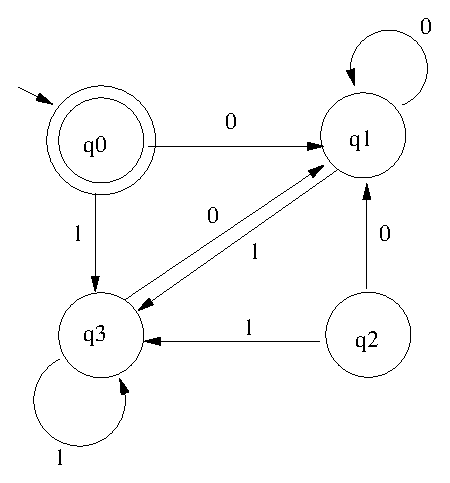
\includegraphics[width=8em]{fig}}
%     \legend{Fonte: Os Autores}
%     \label{fig:ex1}
% \end{figure}

% o `[h]' abaixo é um parâmetro opcional que sugere que o LaTeX coloque a
% figura exatamente neste ponto do texto. Somente preocupe-se com esse tipo
% de formatação quando o texto estiver completamente pronto (uma frase a mais
% pode fazer o LaTeX mudar completamente de idéia sobre onde colocar as
% figuras e tabelas)
% %\begin{figure}[h]
% \begin{figure}
%     \caption{Exemplo de figura desenhada com o environment \texttt{picture}.}
%     \begin{center}
%         \setlength{\unitlength}{.1em}
%         \begin{picture}(100,100)
%                 \put(20,20){\circle{20}}
%                 \put(20,20){\small\makebox(0,0){a}}
%                 \put(80,80){\circle{20}}
%                 \put(80,80){\small\makebox(0,0){b}}
%                 \put(28,28){\vector(1,1){44}}
%         \end{picture}
%     \end{center}
%     \legend{Fonte: Os Autores}
%     \label{fig:ex2}
% \end{figure}

\subsection{Cronograma do Projeto de Pesquisa}

O sucesso na execução de aplicações paralelas em ambientes de Alto Desempenho Computacional (HPC) depende de um conhecimento profundo das tecnologias e ferramentas envolvidas, aliado a uma metodologia rigorosa para testar, avaliar e otimizar tais aplicações. Nesse contexto, a definição de um cronograma de atividades é fundamental para o gerenciamento e a execução sistemática do projeto.

O presente cronograma detalha as diversas fases do projeto de pesquisa sobre o rastreamento de aplicações paralelas com OpenMP, desde a revisão literária inicial até a submissão do artigo final. Através de metas e marcos específicos, busca-se garantir a condução eficiente e dentro do prazo de cada etapa do projeto\\
% Tabelas são construídas com praticamente os mesmos comandos. Ver a tabela \ref{tbl:ex1}.


\begin{table}[h]
	\caption{Cronograma de Atividades para o Estudo do Rastreamento de Aplicações Paralelas com OpenMP}
	\begin{center}
		\begin{tabular}{c|p{10cm}}
			\textbf{Mês} & \textbf{Atividade} \\
			\hline
			\hline
			Abril 2024 & Revisão literária sobre HPC, OpenMP, OMPT, e benchmarks. Preparação do ambiente de teste. Seleção e preparação dos benchmarks. \\
			\hline
			Maio 2024 & Execução dos benchmarks na primeira configuração de hardware (Plataforma Draco). Análise inicial dos dados. Início dos testes na segunda configuração de hardware (Plataforma Hype). \\
			\hline
			Junho 2024 & Continuação dos testes nas configurações de hardware restantes (Plataformas Bleise e Cei). Análise dos dados de todas as configurações. Preparação do relatório inicial dos resultados. \\
			\hline
			Julho 2024 & Finalização do relatório de resultados. Redação e revisão do artigo de pesquisa. Submissão do artigo para revisão. \\
			\hline
		\end{tabular}
	\end{center}
	\legend{Fonte: O Autor}
	\label{tbl:cronograma}
\end{table}


% \subsection{Formato de Figuras}
% \label{sec:fig_format}

% O LaTeX permite utilizar vários formatos de figuras, entre eles \emph{eps}, \emph{pdf}, \emph{jpeg} e \emph{png}. Programas de diagramação como Inkscape (e mesmo LibreOffice) permitem gerar arquivos de imagens vetoriais que podem ser utilizados pelo LaTeX sem dificuldade. Pacotes externos permitem utilizar SVG e outros formatos.

% Dia e xfig são programas utilizados por dinossauros para gerar figuras vetoriais. Se possível, evite-os.

% \subsection{Classificação dos etc.}

% O formato adotado pela ABNT prevê apenas três níveis (capítulo, seção e subseção). Assim, \texttt{\char'134subsubsection} não é aconselhado.

% \section{Sobre as referências bibliográficas}

% A classe \emph{iiufrgs} faz uso do pacote \emph{abnTeX2} com algumas alterações
% feitas por Sandro Rama Fiorini. Culpe ele se algo der errado. Agradeça a ele
% pelo que der certo. As modificações dão uma camada de tinta NATBIB-style,
% já que o abntex2 usa uns comandos de citação feitos para alienígenas de 5 braços
% wtf. Exemplos de citação:

% \begin{itemize}
%     \item \emph{cite}: Unicórnios são verdes \cite{Adams2009Conceptual};
%     \item \emph{citep}:Unicórnios são verdes \citep{Adams2009Conceptual};
%     \item \emph{citet}: Segundo \citet{Adams2009Conceptual}, unicórnios são
%                         verdes.
%     \item \emph{citen or citenum}: Segundo \citen{Adams2009Conceptual},
%         unicórnios são verdes.
%     \item \emph{citeauthor e citeyearpar}: Segundo artigos de
%         \citeauthor{Adams2009Conceptual} , unicórnios são verdes
%         \citeyearpar{Adams2009Conceptual}.

% \end{itemize}

% O estilo abnt fornecido antigamente pelo UTUG não é mais recomendado, pois não
% produz saída de acordo com as exigências da biblioteca.

% Recomenda-se o uso de bibtex para gerenciar as referências (veja o arquivo
% biblio.bib).

% e aqui vai a parte principal
%
% \chapter{Estado da arte}
% \chapter{Mais estado da arte}
% \chapter{A minha contribuição}
% \chapter{Prova de que a minha contribuição é válida}
% \chapter{Conclusão}

% referencias
% aqui será usado o environment padrao `thebibliography'; porém, sugere-se
% seriamente o uso de BibTeX e do estilo abnt.bst (veja na página do
% UTUG)
%
% observe também o estilo meio estranho de alguns labels; isso é
% devido ao uso do pacote `natbib', que permite fazer citações de
% autores, ano, e diversas combinações desses

\bibliographystyle{abntex2-alf}
\bibliography{biblio}

\end{document}
